\documentclass[border=5mm]{standalone}
\usepackage{tikz}
\usetikzlibrary{calc, intersections}

\begin{document}
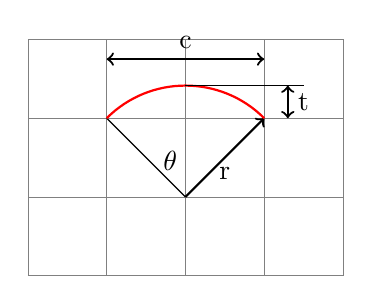
\begin{tikzpicture}

    \draw[help lines] (0,0) grid (4,3);
    \draw [thick,->] (2,1) -- node[below] {r} ++(45:{sqrt(2)});
    \draw (2,1) -- ++(135:{sqrt(2)});
    % Draw the arc which center is (2,1)
    \draw[thick,red] ([shift=(45:{sqrt(2)})]2,1) arc (45:135:{sqrt(2)});
    \draw[thick,<->] (1,2.75) -- node[above] {c} (3,2.75);
    \draw[thin] (2,2.414)-- (3.5,2.414);
    \draw[thick,<->] (3.3,2) -- node[right] {t} (3.3,2.414);
    \node at ($(2,1)+(112.5:0.5)$) {$\theta$};

\end{tikzpicture}
\end{document}

